\documentclass{kspaper}

\title{旅行日记 --- 东京之行}
\author{Kevin Stephen \and Bing}
\date{\today}

\begin{document}

\maketitle

\tableofcontents

\clearpage

\say[ks]{0.64}{本文由 Bing 生成,仅为测试模板使用}

\section{第一天 --- 抵达东京}

\subsection{中文}

我从北京出发,乘坐东方航空的航班,经过四个小时的飞行,终于抵达了东京成田国际机场。
我感到既兴奋又紧张,这是我第一次来到日本,也是我第一次独自出国旅行。
我拿好了我的行李,走出了机场大厅,打算找一辆出租车去酒店。

\subsection{English}

Hello, I departed from Beijing and took a flight from China Eastern Airlines.
After four hours of flying, I finally arrived at Tokyo Narita International Airport.
I felt both excited and nervous, this was my first time to Japan, and also my first time traveling abroad alone.
I picked up my luggage, walked out of the airport hall, and planned to find a taxi to the hotel.

\subsection{日本語}

こんにちは、私は北京を出発し、中国東方航空のフライトに乗りました。
4 時間の飛行の後、ついに東京成田国際空港に到着しました。
私はとても興奮して緊張していました、これは私が初めて日本に来たことで、また私が初めて一人で海外旅行をしたことでした。
私は荷物を受け取り、空港ホールを出て、ホテルに行くためにタクシーを探そうとしました。

\section{第二天 --- 游览浅草寺和东京塔}

\subsection{中文}

第二天早上,我吃了一个简单的早餐,就出发去游览东京的名胜古迹。
我首先去了浅草寺,这是一座有着悠久历史的佛教寺院,建于公元 645 年。
浅草寺的门前有一条热闹的商业街,叫做 ``仲见世通り'',我在那里买了一些纪念品和小吃,还试了一下占卜。
浅草寺的建筑非常壮观,尤其是雷门和五重塔,让我感受到了日本传统文化的魅力。

\subsection{English}

On the second morning, I had a simple breakfast and set off to visit the famous historical sites in Tokyo.
I first went to Sensoji Temple, which is a Buddhist temple with a long history, built in 645 AD.
In front of the gate of Sensoji Temple, there is a lively commercial street called Nakamise-dori,
where I bought some souvenirs and snacks, and also tried fortune-telling.
The architecture of Sensoji Temple is very magnificent, especially the Kaminarimon Gate and the Five-storied Pagoda,
which made me feel the charm of Japanese traditional culture.

\subsection{日本語}

2 日目の朝、私は簡単な朝食をとって、東京の有名な歴史的な場所を見に出かけました。
私はまず浅草寺に行きました、これは長い歴史を持つ仏教寺院で、645 年に建てられました。
浅草寺の門の前には、仲見世通りという賑やかな商店街があります、私はそこでいくつかのお土産やおやつを買ったり、占いを試したりしました。
浅草寺の建築はとても壮大で、特に雷門と五重塔は、私に日本の伝統文化の魅力を感じさせました。

\section{第三天 --- 参观东京迪士尼乐园}

\subsection{中文}

第三天是我最期待的一天,因为我要去东京迪士尼乐园玩。
东京迪士尼乐园是日本最受欢迎的主题公园之一,也是全球最大的迪士尼乐园之一。
我早早地到了公园的入口,拿到了门票,就开始了我的奇妙之旅。
我玩了很多有趣的项目,比如小飞象、海盗船、白雪公主城堡等,还看了精彩的游行和烟花表演。
我觉得自己像一个孩子一样,忘记了所有的烦恼,只享受着快乐。

\subsection{English}

The third day was the day I was looking forward to the most, because I was going to Tokyo Disneyland.
Tokyo Disneyland is one of the most popular theme parks in Japan, and also one of the largest Disneylands in the world.
I arrived at the entrance of the park early, got my ticket, and started my wonderful journey.
I played a lot of fun attractions, such as Dumbo, Pirates of the Caribbean, Snow White's Castle, etc.,
and also watched amazing parades and fireworks shows.
I felt like a child, forgetting all my troubles, and just enjoying the happiness.

\subsection{日本語}

3日目は私が一番楽しみにしていた日でした、なぜなら私は東京ディズニーランドに行くからです。
東京ディズニーランドは日本で最も人気のあるテーマパークの一つであり、世界で最も大きなディズニーランドの一つでもあります。
私は早くにパークの入り口に着き、チケットを手に入れ、私の素晴らしい旅を始めました。
私はたくさんの楽しいアトラクションを楽しみました、例えばダンボ、カリブの海賊、白雪姫の城など、そして素晴らしいパレードや花火ショーも見ました。
私は子供のように感じました、すべての悩みを忘れて、ただ幸せを楽しんでいました。

\section{第四天 --- 离开东京}

\subsection{中文}

第四天是我在东京的最后一天,我收拾好了我的行李,准备离开酒店。
我在酒店的前台办理了退房手续,然后搭乘了机场巴士去机场。
在巴士上,我回顾了这几天在东京的经历,觉得非常充实和难忘。
我对东京这座城市有了更深的了解和喜爱,也结识了一些新的朋友。
我希望有一天能再来东京,探索更多的美好。

\subsection{English}

The fourth day was my last day in Tokyo, I packed my luggage and prepared to leave the hotel.
I checked out at the front desk of the hotel, and then took the airport bus to the airport.
On the bus, I reviewed my experience in Tokyo for the past few days, and felt very fulfilled and unforgettable.
I had a deeper understanding and love for Tokyo, and also made some new friends.
I hope to come back to Tokyo someday, and explore more beauty.

\subsection{日本語}

4日目は私が東京にいる最後の日でした、私は荷物をまとめてホテルを出る準備をしました。
私はホテルのフロントでチェックアウトを済ませ、空港バスに乗って空港に向かいました。
バスの中で、私はこの数日間の東京での経験を振り返り、とても充実して忘れられないものだと感じました。
私は東京という街に対してより深い理解と愛情を持ちましたし、新しい友達もできました。
いつかまた東京に来て、もっと美しいものを探索できることを願っています

\section{代码测试}

下面部分是我的一些代码测试,测试代码渲染效果:

\begin{table}[H]
    \begin{minted}[mathescape]{rust}
// 代码解释
// $fib(0) = 0$
// $fib(1) = 1$
// $fib(n) = fib(n - 1) + fib(n - 2)$
pub fn fib(n: usize) -> usize {
    fn fib_cache(n: usize, a: usize, b: usize) -> usize {
        match n {
            0 => a,
            1 => b,
            _ => fib_cache(n - 1, b, a + b),
        }
    }
    fib_cache(n, 0, 1)
}

fn main() {
    println!("fib 20 = {}", fib(20));
}
    \end{minted}
    \caption{rust代码:斐波那契数列}
    \label{code:rust-fib}
\end{table}

对应 代码\ref{code:rust-fib} 的执行效果如 图\ref{fig:rust-fib} 所示:

\begin{figure}[H]
    \centering
    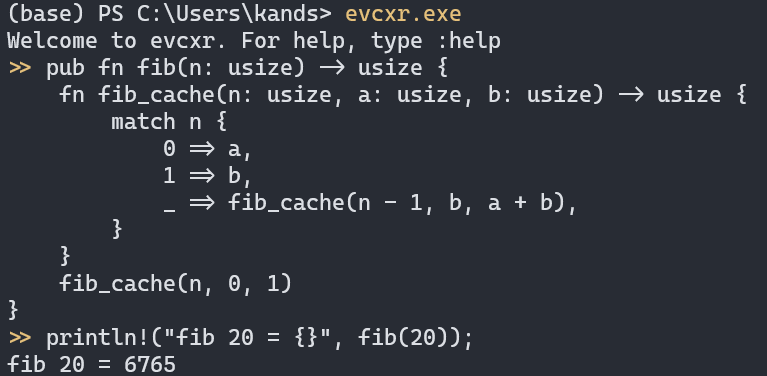
\includegraphics[scale=0.64]{pics/rust-fib.png}
    \caption{代码演示:rust --- 斐波那契数列}
    \label{fig:rust-fib}
\end{figure}

\end{document}